
\section{Sensor Setup}

\subsection{Light Curtain Basics}

\begin{figure}[h]
   \centering
   \begin{minipage}{0.5\textwidth}
       \centering
       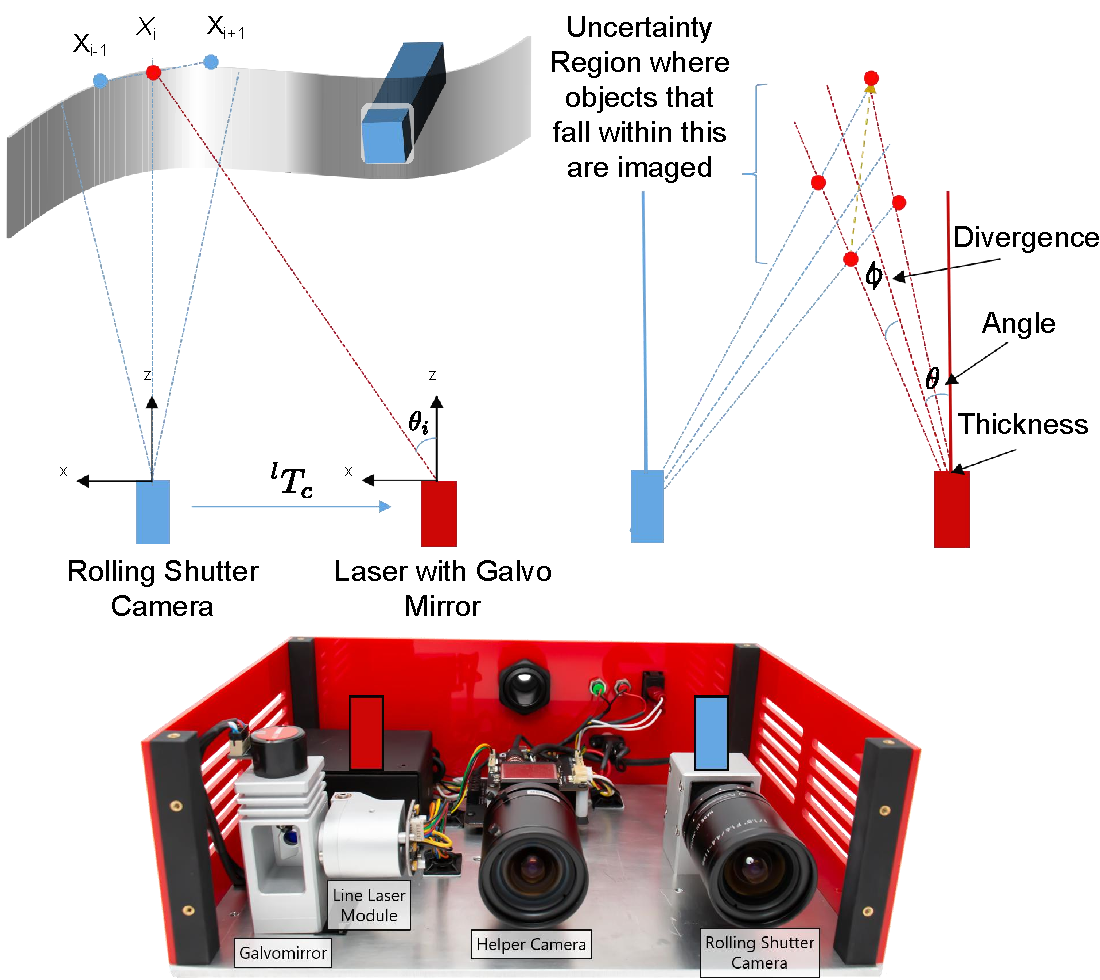
\includegraphics[width=1.0\textwidth]{figures/LC.pdf} % first figure itself
   \end{minipage}\hfill
   % \begin{minipage}{0.3\textwidth}
   %     \centering
   %     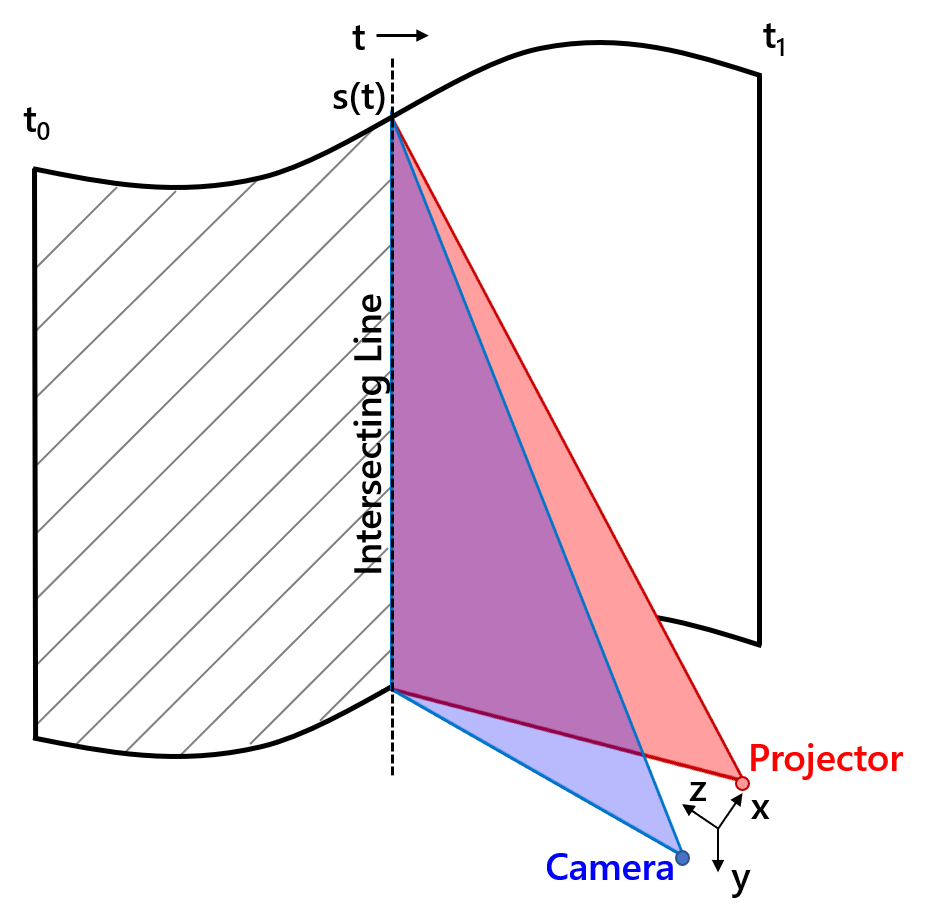
\includegraphics[width=0.9\textwidth]{light_curtain_iso.png} % second figure itself
   % \end{minipage}
   \centering
   \caption{The Programmable Light Curtain device, consisting of a steerable laser, an IR camera and a microcontroller, capable of generating a slice in space to image in 3D}
\end{figure}

The Light Curtain consists of a rolling shutter NIR camera flipped vertically, a Line Laser module and a Galvomirror. The rolling shutter NIR camera runs in sync with the laser, where each row of the camer can be thought of as a plane with some divergence going out vertically into space. The laser/projector fires a similar vertical sheet of light as a plane into space, which intersects with the camera's vertical plane to produce an intersecting volume. We call this the \textit{thickness} of the curtain. Any objects that lie within this space will then be imaged by the camera. We we will know the 3D position of said objects. Hence, a top-down XZ profile can be provided in the NIR camera's frame, to generate a ruled 3D curtain surface at ~50fps

\subsection{Simulator}

\begin{figure}[h]
   \centering
   \begin{minipage}{0.5\textwidth}
       \centering
       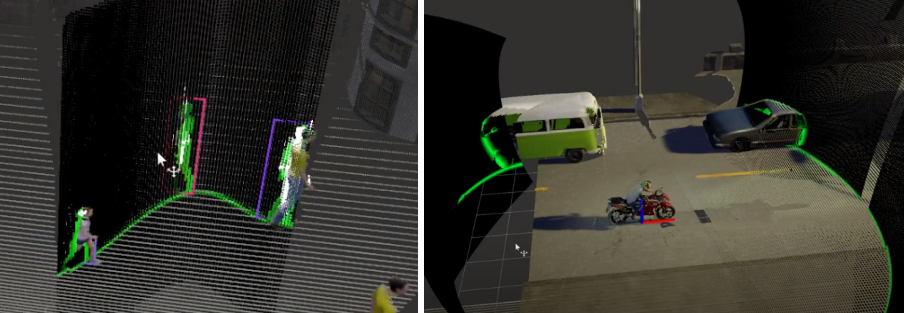
\includegraphics[width=1.0\textwidth]{figures/sim.png}
   \end{minipage}\hfill
   \centering
   \caption{Light Curtain Simulator in CARLA environment}
\end{figure}

We also designed and open sourced a light curtain simulator to test and evaluate our algorithms, allowing for the Light Curtain paramters such as NIR instrinsics, Laser/NIR extrinsincs, Galvomirror speed etc. to be controlled.

\subsection{Sensor Array}

\begin{figure}[h]
   \centering
   \begin{minipage}{0.5\textwidth}
       \centering
       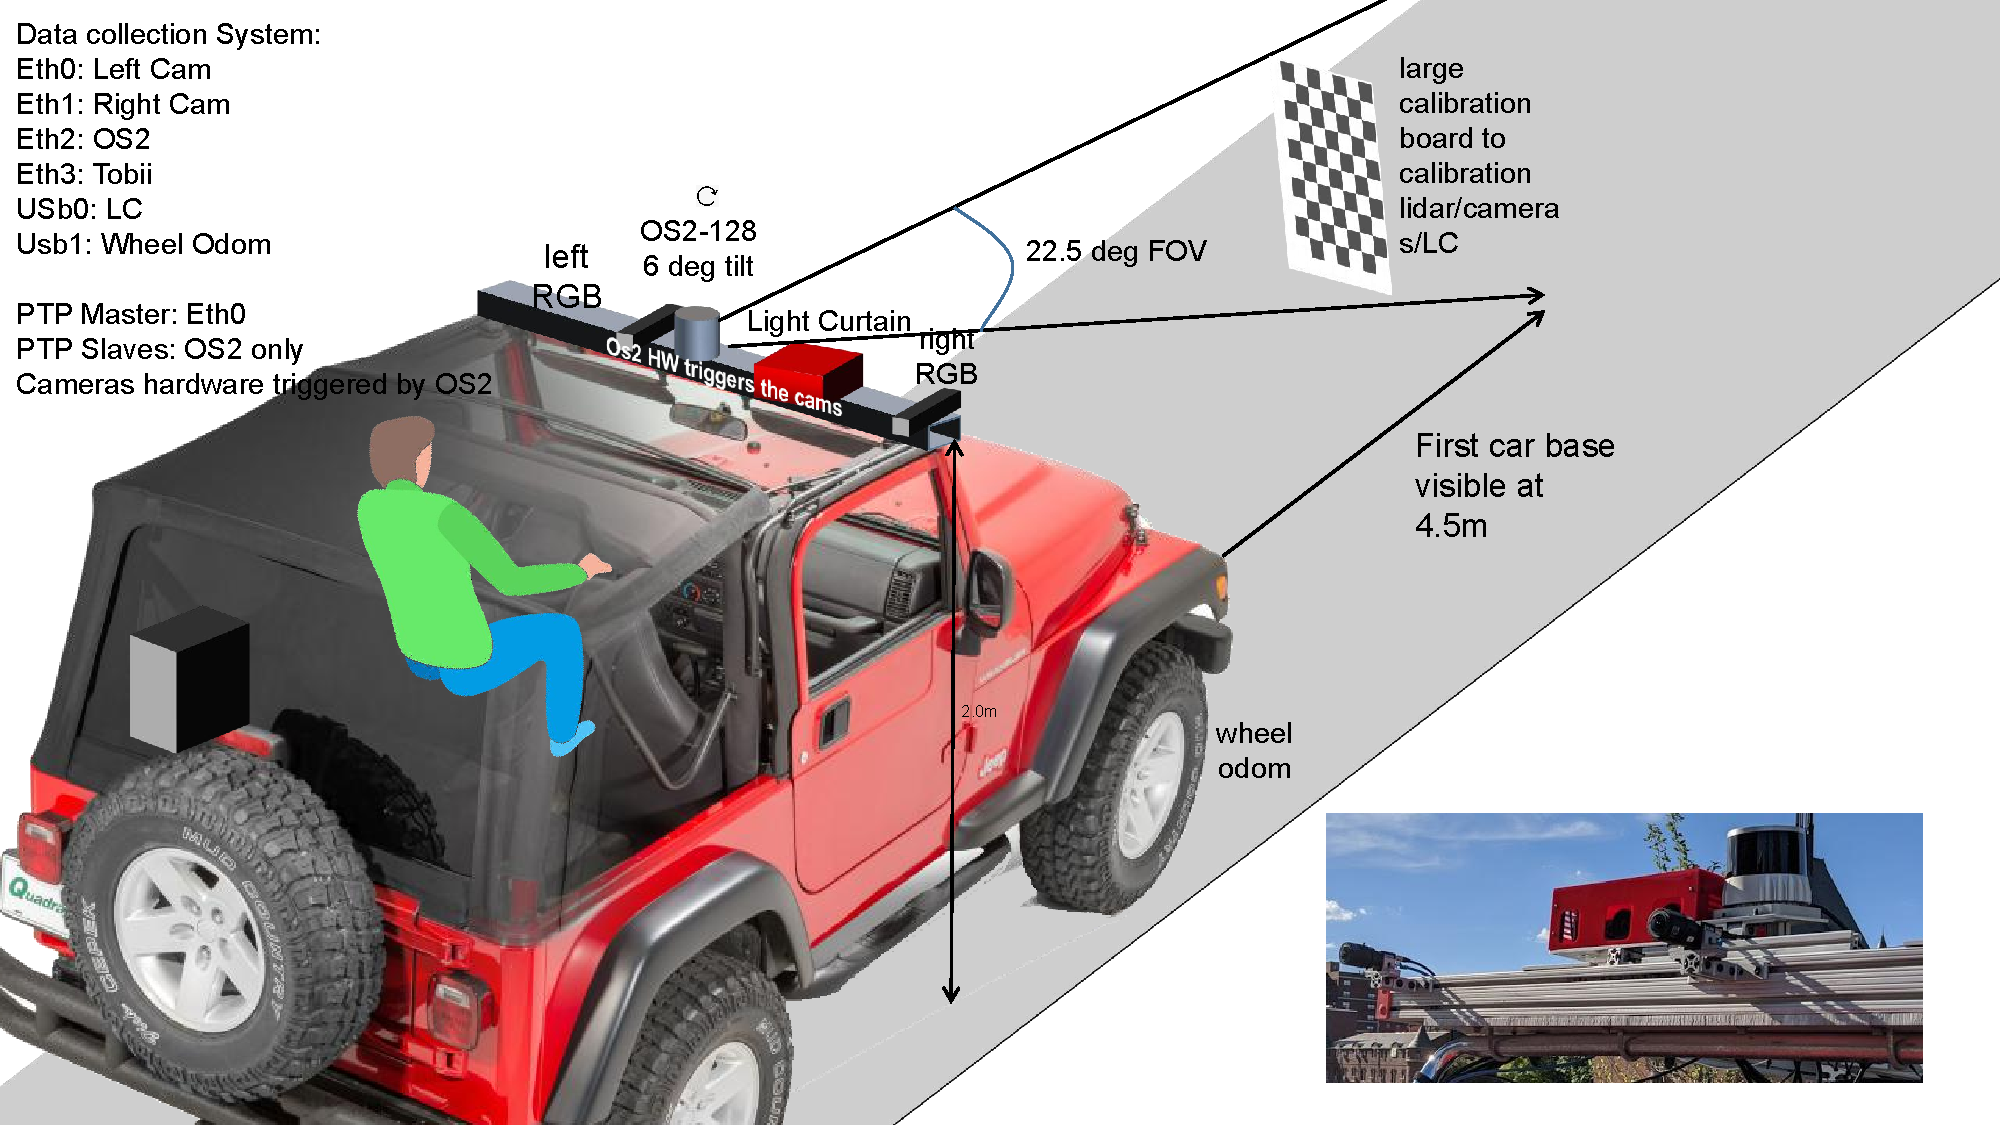
\includegraphics[width=1.0\textwidth]{figures/array.pdf}
   \end{minipage}\hfill
   \centering
   \caption{Sensor Array consisting of a Stereo camera pair, the Light Curtain device and a 128 Beam Lidar}
\end{figure}

Our sensor array consists of a Stereo Camera Pair with a baseline of 0.7m, the Light Curtain device located close to the main/left camera to minimize depth/volume transformation parallax artifacts, and an Ouster OS2-128 Lidar for algorithm accuracy validation and to assist in training depth estimation networks. All sensors are calibrated to the common reference frame of the left RGB camera.